\documentclass[11pt]{article}

% ---- SPIE Manuscript margin spec (Letter): 0.88in L/R, 1.0in top, 1.25in bottom ----
\usepackage[letterpaper, left=0.88in, right=0.88in, top=1.0in, bottom=1.25in]{geometry}

\usepackage{times}
\usepackage[T1]{fontenc}
\usepackage{graphicx}
\usepackage{booktabs}
\usepackage{amsmath}
\usepackage[colorlinks=true, linkcolor=black, citecolor=black, urlcolor=black]{hyperref}
\usepackage{caption}
\usepackage{titlesec}
\usepackage{enumitem}

\titlespacing*{\section}{0pt}{10pt}{4pt}
\titlespacing*{\subsection}{0pt}{8pt}{3pt}
\setlist[itemize]{topsep=2pt, itemsep=1pt, parsep=0pt}

\title{\vspace{-1.5em}\Large\bfseries Does Medical Pretraining Change What a Chest-Radiograph Classifier Needs?\\[2pt] A Frozen-Protocol Comparison on CheXpert}

% ---- FILL IN: author names, affiliations, contact ----
\author{
  [Author Name(s)]\textsuperscript{a} \\[2pt]
  \small \textsuperscript{a}[Affiliation, Department, Institution, City, State/Country] \\
  \small Corresponding author: [email]
}
\date{}

\begin{document}
\maketitle
\vspace{-2em}

\section*{Purpose}

Chest-radiograph classifiers are conventionally reported by AUC or overall accuracy, metrics that can conceal a severe, clinically disqualifying failure mode on a long-tailed, multi-label diagnostic task: a model can score highly on accuracy while missing most true positives. Large-scale medical pretraining --- exemplified by Ark+ \cite{ma2025ark}, trained across six chest-radiograph datasets --- is increasingly used to build chest X-ray foundation models, but it remains unclear whether such pretraining actually changes what a classifier \emph{needs}: how long it must train before overfitting, how well-calibrated its raw outputs are, and whether it still benefits from long-tail-aware loss design once large-scale pretraining is present. This work asks those three questions directly, under a single frozen protocol, rather than proposing a new architecture or loss.

\section*{Methods}

We compare six chest-radiograph classification architectures on CheXpert \cite{irvin2019chexpert}: Ark+ (Swin-Large \cite{liu2021swin}, large-scale medical pretraining), an architecture-matched no-pretraining control (Swin-Large, random init --- isolating the effect of pretraining with architecture held fixed), Swin Transformer V2 Base \cite{liu2022swinv2} (ImageNet-22k), DenseNet-121 \cite{huang2017densenet} (ImageNet-1k), RAD-DINO \cite{perezgarcia2025raddino} (DINOv2 ViT-B/14), and ConvNeXt V2 Base \cite{woo2023convnextv2} (ImageNet-22k). Ark+'s three original task-specific components (per-class uncertain-label strategy, class-weighted loss, co-occurrence regularization) are stripped so that all six models are evaluated under one identical recipe, listed in Table~\ref{tab:protocol}.

\begin{table}[h]
\centering
\small
\caption{Frozen training protocol, identical across all six architectures.}
\label{tab:protocol}
\begin{tabular}{@{}ll@{}}
\toprule
Setting & Value \\
\midrule
Input resolution & $320\times320$ (native CheXpert-small short side) \\
Optimizer & AdamW, cosine schedule, 1 warmup epoch, lr $5\times10^{-5}$, wd $0.05$ \\
Epochs & 30, checkpoint selected by best \emph{validation} macro-AUC \\
Validation set & Official CheXpert \texttt{valid.csv} (234 studies) \\
Test set & Patient-disjoint held-out (15\% of patients), touched once, after training \\
Uncertain labels & U-Zeros (headline); U-Ones as an appendix sensitivity check \\
Seeds & 2 for headline results (13, 42), 1 for screening \\
Metrics & Macro-AUC, F1, sensitivity, accuracy, MCC, AP, ECE \\
\bottomrule
\end{tabular}
\end{table}

Three questions are asked of this shared design: (a) \emph{does pretraining delay overfitting}, isolated cleanly via the Ark+/Swin-Large architecture-matched pair (pretraining is the only variable); (b) \emph{does pretraining produce a better-calibrated model}, and does per-label operating-point (threshold, selected by Youden's $J$ statistic \cite{youden1950index}) policy close the accuracy--sensitivity gap that raw AUC hides; (c) \emph{do large-scale-pretrained encoders still need long-tail-aware loss}, tested architecture-conditionally across all six models. Threshold policies and temperature calibration \cite{guo2017calibration} are fit on the validation set only and applied once to the held-out test set, avoiding the leakage that results from tuning a threshold on the same set it is then evaluated on.

\section*{Results (preliminary)}

Ark+'s headline result is complete: Table~\ref{tab:results} reports held-out test performance across the five CheXpert competition classes (Atelectasis, Cardiomegaly, Consolidation, Edema, Pleural Effusion), mean $\pm$ std over 2 seeds.

\begin{table}[h]
\centering
\caption{Ark+ held-out test performance, mean $\pm$ std over 2 seeds (13, 42).}
\label{tab:results}
\resizebox{\textwidth}{!}{%
\begin{tabular}{@{}lccccccc@{}}
\toprule
 & AUC & F1 & Sensitivity & Accuracy & MCC & AP & ECE \\
\midrule
Ark+ & $0.806\pm0.003$ & $0.472\pm0.005$ & $0.783\pm0.004$ & $0.705\pm0.008$ & $0.369\pm0.006$ & $0.480\pm0.004$ & $0.013\pm0.002$ \\
\bottomrule
\end{tabular}%
}
\end{table}

\noindent The Sensitivity column already reflects the validation-tuned Youden's-J operating point, not the naive 0.5 threshold. Figure~\ref{fig:threshold} shows why that choice matters: at the naive 0.5 threshold, Ark+ reaches 0.86 accuracy but only 0.29--0.32 mean sensitivity --- missing roughly seven in ten true positives despite a high headline accuracy. A validation-tuned threshold (Youden's J or F1-optimal) recovers sensitivity to 0.73--0.84 at a real but bounded accuracy cost, at \emph{unchanged} AUC, since AUC is threshold-independent. Both seeds show this pattern with near-identical magnitude, indicating it is not an artifact of one run.

\begin{figure}[h]
\centering
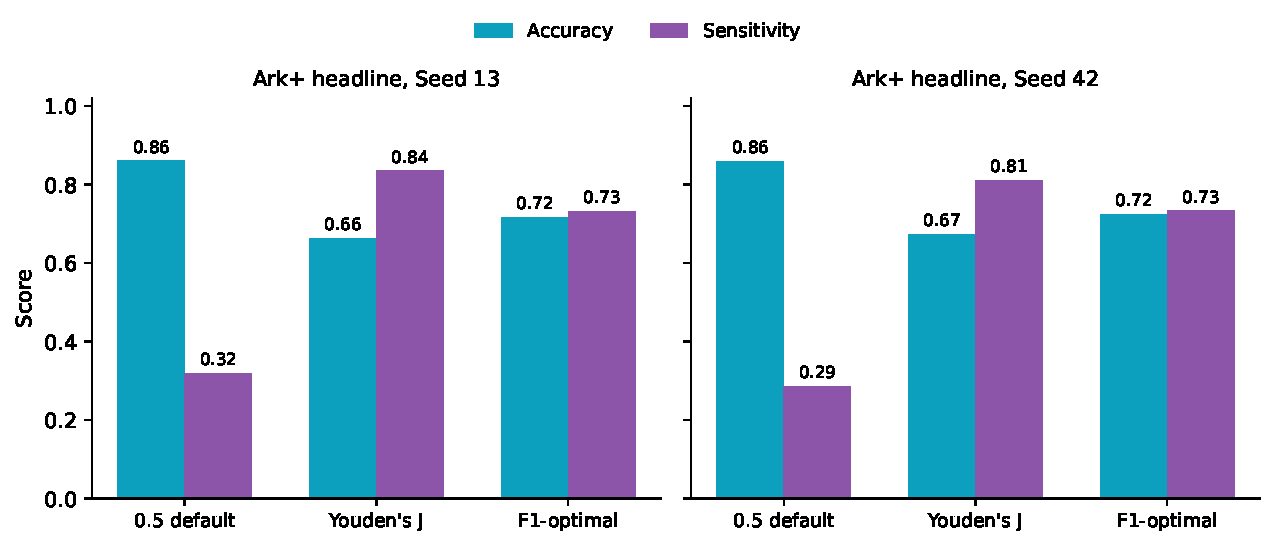
\includegraphics[width=0.95\textwidth]{fig_threshold_policy.pdf}
\caption{Accuracy vs.\ sensitivity by threshold policy, Ark+ held-out test, both headline seeds. Thresholds and calibration are fit on validation only and applied once to test.}
\label{fig:threshold}
\end{figure}

A single global temperature-scaling calibration, also fit on validation, did \emph{not} improve held-out calibration in this preliminary result (ECE increased from $\approx$0.011--0.015 to $\approx$0.070 after scaling); the fitted temperature ($T\approx1.6$) over-corrected a model whose raw outputs were already reasonably well-calibrated on this split. We report this as a genuine negative finding, likely attributable to the small (234-image) official validation set, rather than omit it.

Training for the remaining five architectures --- including the Ark+/Swin-Large controlled pretraining comparison central to question (a) --- and the architecture-conditional loss-design analysis for question (c) are in progress under the identical frozen protocol above and will be presented at the conference.

\section*{Novel and Breakthrough Aspects}

To our knowledge this is among the first independent evaluations of Ark+ (published June 2025) that isolates the effect of its large-scale pretraining from its architecture via a matched no-pretraining control, rather than comparing it only against unrelated architectures. The threshold-policy result in Figure~\ref{fig:threshold} makes a specific, quantitative version of a widely-suspected but rarely-isolated claim: that headline accuracy on CheXpert-scale long-tailed data can be nearly independent of clinically-relevant sensitivity, and that this gap is substantially --- though not fully --- closeable without any additional training, purely through validation-tuned operating-point selection.

\section*{Related Work}

CheX-DS \cite{chexds2025} ensembles DenseNet and a Swin Transformer with a weighted BCE plus asymmetric loss on NIH ChestX-ray14, reporting 83.76\% average AUC. Our work differs in dataset (CheXpert vs.\ ChestX-ray14), in scope (six architectures under one frozen protocol vs.\ one proposed ensemble), and in framing: we do not propose an ensembling method or claim novelty for asymmetric loss itself; question (c) instead asks, architecture-conditionally, whether large-scale pretraining already absorbs the long-tail imbalance that motivates such losses in the first place. A DenseNet-121/Ark+ logit-fusion analysis is planned as a subordinate diagnostic, not a headline contribution, given CheX-DS's prior ensemble result.

\section*{Conclusion}

Under identical protocol conditions, Ark+ shows a large, real gap between headline accuracy and clinically-relevant sensitivity that validation-tuned thresholding substantially recovers at no AUC cost --- but naive single-temperature calibration on a small validation set did not help, and may hurt. Whether large-scale medical pretraining changes training length, calibration behavior, or long-tail loss requirements relative to architecture-matched and ImageNet-pretrained baselines is being tested directly via the controlled comparisons above; full six-architecture results will be presented.

\section*{Disclosure of Prior or Concurrent Submissions}

[FILL IN --- required field. State here whether this work, or any subset of it, has been submitted, presented, or published elsewhere, or state that it has not.]

\bibliographystyle{plain}
\begin{thebibliography}{9}

\bibitem{ma2025ark}
D.~Ma, J.~Pang, M.~B.~Gotway, and J.~Liang,
``A fully open AI foundation model applied to chest radiography,''
\emph{Nature}, 2025.

\bibitem{irvin2019chexpert}
J.~Irvin, P.~Rajpurkar, M.~Ko, et al.,
``CheXpert: A large chest radiograph dataset with uncertainty labels and expert comparison,''
\emph{Proc. AAAI Conf. Artificial Intelligence}, 33(1), 590--597, 2019.

\bibitem{chexds2025}
X.~Li, Y.~Liu, X.~Xu, and X.~Zhao,
``CheX-DS: Improving Chest X-ray Image Classification with Ensemble Learning Based on DenseNet and Swin Transformer,''
arXiv:2505.11168, 2025.

\bibitem{guo2017calibration}
C.~Guo, G.~Pleiss, Y.~Sun, and K.~Q.~Weinberger,
``On calibration of modern neural networks,''
\emph{Proc. Int. Conf. Machine Learning (ICML)}, 2017.

\bibitem{liu2021swin}
Z.~Liu, Y.~Lin, Y.~Cao, H.~Hu, Y.~Wei, Z.~Zhang, S.~Lin, and B.~Guo,
``Swin Transformer: Hierarchical vision transformer using shifted windows,''
\emph{Proc. IEEE/CVF Int. Conf. Computer Vision (ICCV)}, 2021.

\bibitem{liu2022swinv2}
Z.~Liu, H.~Hu, Y.~Lin, Z.~Yao, Z.~Xie, Y.~Wei, J.~Ning, Y.~Cao, Z.~Zhang, L.~Dong, F.~Wei, and B.~Guo,
``Swin Transformer V2: Scaling up capacity and resolution,''
\emph{Proc. IEEE/CVF Conf. Computer Vision and Pattern Recognition (CVPR)}, 2022.

\bibitem{huang2017densenet}
G.~Huang, Z.~Liu, L.~van~der~Maaten, and K.~Q.~Weinberger,
``Densely connected convolutional networks,''
\emph{Proc. IEEE Conf. Computer Vision and Pattern Recognition (CVPR)}, 2017.

\bibitem{woo2023convnextv2}
S.~Woo, S.~Debnath, R.~Hu, X.~Chen, Z.~Liu, I.~S.~Kweon, and S.~Xie,
``ConvNeXt V2: Co-designing and scaling ConvNets with masked autoencoders,''
arXiv:2301.00808, 2023.

\bibitem{perezgarcia2025raddino}
F.~P\'erez-Garc\'ia, H.~Sharma, S.~Bond-Taylor, K.~Bouzid, V.~Salvatelli, M.~Ilse, S.~Bannur, D.~C.~Castro, A.~Schwaighofer, M.~P.~Lungren, M.~T.~Wetscherek, N.~Codella, S.~L.~Hyland, J.~Alvarez-Valle, and O.~Oktay,
``Exploring scalable medical image encoders beyond text supervision,''
\emph{Nature Machine Intelligence}, 2025.

\bibitem{youden1950index}
W.~J.~Youden,
``Index for rating diagnostic tests,''
\emph{Cancer}, 3(1), 32--35, 1950.

\end{thebibliography}

\end{document}
